% $HeadURL$

%%%%%%%%%%%%%%%%%%%%%%%%%%%%%%%%%%%%%%%%%%%%%%%%%%%%%%%%%%%%%%%%%%%%%%
%%                     Subunit
%%%%%%%%%%%%%%%%%%%%%%%%%%%%%%%%%%%%%%%%%%%%%%%%%%%%%%%%%%%%%%%%%%%%%%

\subsection{Glyph\add{s}: \glyph{Subunits}}
\label{sec:subunit}

\corr{The \glyph{subunit} is used to describe the composition of the \glyph{complex}.
A \glyph{complex} can optionally be decorated with one or more subunits, which represent the types of \corr{\glyph{EPN}}{entities} that may aggregate to form a \glyph{complex}.
A \glyph{subunit} is an auxiliary unit that decorates the \glyph{complex} and does not represent or mimic an \glyph{EPN} directly, it only indicates the type of subunit included in the \glyph{complex}.
The example in \fig{complexSubunits} illustrates the use of \glyph{subunits} in a \glyph{complex}.
It also shows an equivalent complex without subunits.
}
{
A complex is formed by the non-covalent binding of two or more entities, that become the subunits of the complex.
In \PD, the composition of a complex may be described using \glyph{subunit} glyphs, that are auxiliary units decorating \glyph{complexes}.
\glyph{Subunits} do not represent or mimic entity pools~(\sect{EPNs}) and may only be used to represent the subunits included in a complex.
The example in \fig{complexSubunits} illustrates the use of \glyph{subunits} to describe the composition of a complex.
It also shows how the same complex can be represented without decorating \glyph{subunits}.
}

\add{
The SBGN \PD defines nine different \glyph{subunit} glyphs, each representing a different type of bio-molecular (sub)-entity.
The five main \glyph{subunits} are the \glyph{unspecified entity subunit}, \glyph{macromolecule subunit}, \glyph{simple chemical subunit}, \glyph{nucleic acid feature subunit}, and \glyph{complex subunit}.
\rougny{Maybe no need to list all subunits?}
This latter \glyph{subunit} allows representing complexes formed of other complexes.
The remaining four \glyph{subunits} are multimeric: \glyph{multimer of macromolecules subunit}, \glyph{multimer of simple chemicals subunit}, \glyph{multimer of nucleic acid feature subunit}, and \glyph{multimer of complexes subunit}.
}

\begin{glyphDescription}

\glyphSboTerm
Not applicable.

\add{
\glyphIncoming
None.
}

\add{
\glyphOutgoing
None.
}
\rougny{Is this true? No modulation arcs can depart from subunits inside complexes?
I'm pretty sure I've seen this in some maps though.}
% \corr{The symbol used for the}{The shape of used to represent a} \glyph{subunit} \corr{glyph}{} varies depending on the \glyph{subunit} type.
% The available \corr{symbols}{shapes} are equivalent to those used by the \glyph{EPN} glyphs (see \sect{EPNs})\add{,} including the \glyph{complex}.
% Therefore it is possible to describe complexes within complexes. The mapping between \corr{these and the symbol}{the \glyph{subunit} types and the containers to be used} is shown in the \tab{subunit_containers} below.
% }{
\glyphContainer
\add{Each \glyph{subunit} is represented by \corr{a different}{its own} shape depending on its bio-molecular nature, as shown in \tab{subunit_containers}.\blinov{Shapes may be identical.}
Those shapes are the same as those used to represent entity pools~(\sect{EPNs}).
\corr{However, \glyph{subunits} do not represent the same concepts, and can be seen as ``homonyms''.}{}}\blinov{Homonyms are never defined.}
% }

\luna{032819 replace string of characters with character string}
\corr{\glyphLabel A \glyph{subunit} is identified by a label that is \corr{an unbordered box containing}{} a string of characters \corr{.
The characters}{that} can be distributed on several lines to improve readability. \corr{, although this is not mandatory}{}.
The centre of the label box must be attached to the centre of the container.
The label may spill outside of the container.
}
{
\glyphLabel
A \glyph{subunit} is identified by a label that is \corr{an unbordered box containing}{} a string of characters \corr{.
The characters}{that} can be distributed on several lines to improve readability.
\dogrusoz{how about we simply say: "The characters may be distributed on several lines to improve readability." Not mandatory part is redundant I think.\\
AR: done for all glyphs}
The centre of the label must be placed on the centre of the \corr{shape}{container}.
The label may extend outside of the \corr{shape}{container}.
}


\add{\glyphAux A \glyph{subunit} may carry auxiliary units, depending on its type.}

\add{A \glyph{macromolecule}, \glyph{nucleic acid feature}, or \glyph{complex subunit} can carry one or more \glyph{state variables} that add information about its state (\sect{stateVariable}).
The state of such a \glyph{subunit} is defined as the set of all its \glyph{state variables}.}

\add{A \glyph{macromolecule}, \glyph{simple chemical}, \glyph{nucleic acid feature}, or \glyph{complex subunit} can carry one or more \glyph{units of information} (\sect{unitInfo}).
These can characterize a domain, such as a binding site.
Particular \glyph{units of information} are available for describing the material type (\sect{material-types-cv}) and conceptual type (\sect{conceptual-types-cv}) of such a \glyph{subunit}}.

\end{glyphDescription}

\begin{table}[h]
\begin{tabu}{X[c,m]X[c,m]X[c,m]X[c,m]}
    \toprule
    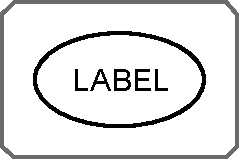
\includegraphics[scale = 0.8, valign = m]{images/unspecified-subunit} & 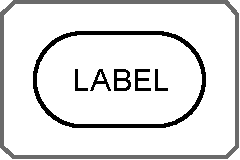
\includegraphics[scale = 0.8, valign = m]{images/simple_chemical-subunit} & 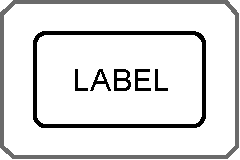
\includegraphics[scale = 0.8, valign = m]{images/macromolecule-subunit} & 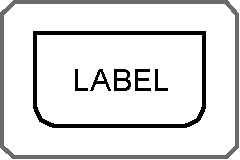
\includegraphics[scale = 0.8, valign = m]{images/genetic-subunit}\\[0.2cm]
    \glyph{unspecified entity subunit} & \glyph{simple chemical subunit} & \glyph{macromolecule subunit} & \glyph{nucleic acid feature subunit}\\[0.5cm]
    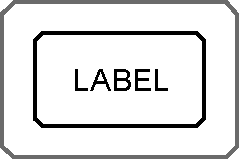
\includegraphics[scale = 0.8, valign = m]{images/complex-subunit} & 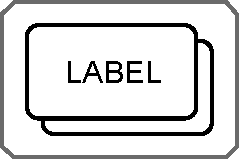
\includegraphics[scale = 0.8, valign = m]{images/macromolecule-multimer-subunit} & 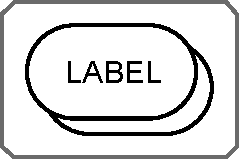
\includegraphics[scale = 0.8, valign = m]{images/simple_chemical-multimer-subunit} & 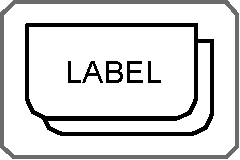
\includegraphics[scale = 0.8, valign = m]{images/genetic-multimer-subunit}\\[0.2cm]
    \glyph{complex subunit} & \glyph{multimer of macromolecules subunit} & \glyph{multimer of simple chemicals subunit} & \glyph{multimer of nucleic acid feature subunit}\\[0.5cm]
    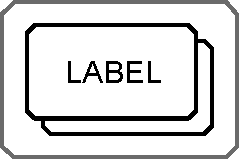
\includegraphics[scale = 0.8, valign = m]{images/complex-multimer-subunit} &  &  & \\[0.2cm]
    \glyph{multimer of complexes subunit} & & & \\
    \bottomrule
\end{tabu}
\caption{The \PD glyphs for the different types of \glyph{subunits}.
Each \glyph{subunit} decorates a \glyph{complex}.}
\label{tab:subunit_containers}
\end{table}


\begin{figure}[htb]
  \centering
  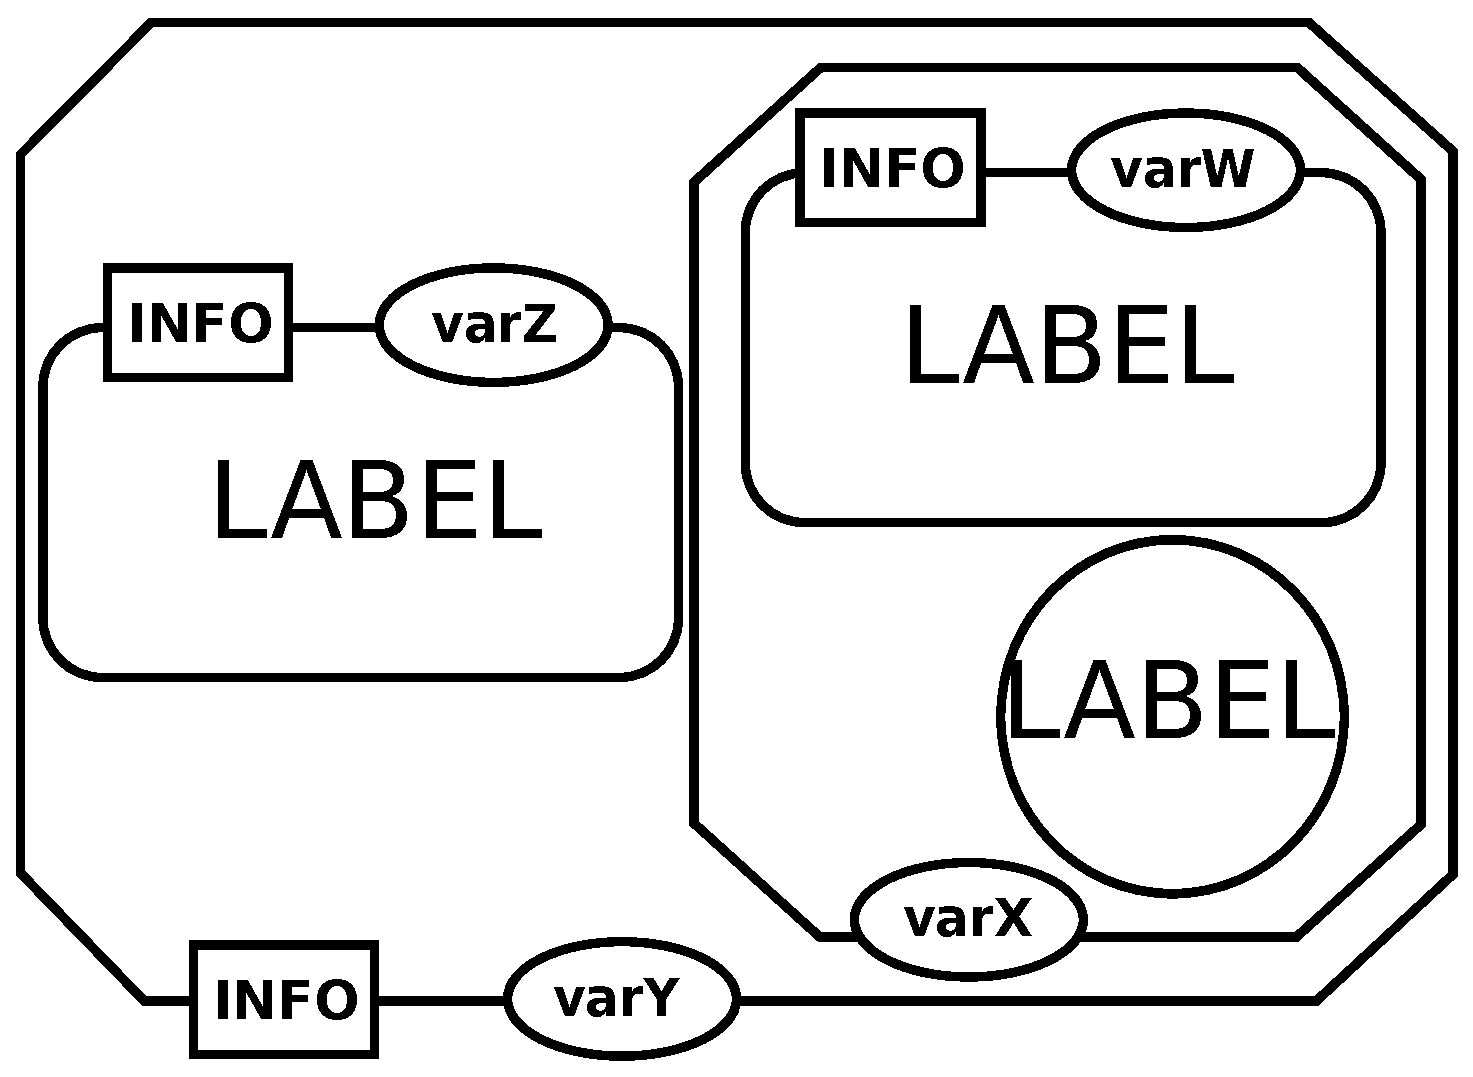
\includegraphics[scale=0.8]{images/complex}
  \caption{Both these complex glyphs are equivalent.
      The \corr{one}{complex} on the left is described using \glyph{subunit} decorators\corr{, the one}{.}
      \add{The complex} on the right depicts the same information, \corr{without them}{without explicitly representing those subunits, that are only suggested by the label of the \glyph{complex}.
  However, their states are represented using \glyph{state variables} decorating the \glyph{complex}.}}
  \label{fig:complexSubunits}
\end{figure}


